\chapter{Related Work}
\label{ch:related}


%In this chapter, we focus on previous work that is related to the problem stated in \nameref{ch:introduction}. 
In this chapter, we discuss the related work to our problem, i.e., research that has been realized in the field of RDF syntax parsing and checking.

\section{RDF Parsing and Syntax Checking}

There exist several tools for validating RDF data as an input.
Ontology engineers can either use tools that are available online or can download desktop applications for syntax validation.
These tools  can commonly detect only the first error while consecutively parsing input from its start point to its end. 
Therefore, semantic developers and engineers are struggling whilst debugging their RDF data, and they need alternative tools that could be more helpful. 
To the best of our knowledge, there is no fault-tolerant tool for parsing and syntax checking various RDF serializations which can detect multiple errors at the same time.  
Hence, a tool that can prominently list all errors included in the RDF data is of paramount importance.

\subsection{RDF/XML Parsing Tools}

Despite the existence of several theoretical models and practical tools that have been invented in the same field, we can hardly find  research that cares for finding more than one syntax error inside RDF data. 
During our journey of searching the existing tools that provide such a service, the W3C RDF validation tool \cite{W3C:Validation:Online} was firstly checked.
It is a web tool available online for the purpose of parsing and validating RDF/XML codes. 
It uses an Another RDF Parser (ARP) parser of Jena \cite{McBride:2002:JSW:613357.613755} as its core; However, it fails in detection of multiple syntax errors and shows only the first encountered error as it is shown in Figure \ref{Fig:errorW3RDFValidator}.
 
In 2000, a Validating RDF Parser (VRP) \cite{karsten:Thesis:2000} was developed by K. Tolle. In his thesis, 
VRP is a Java-based parsing tool with included features for semantically and syntactically checking dedicated for RDF/XML format. 
Nevertheless, the validation functionality provided by VRP is limited to parse only a format type of RDF/XML and does not support other RDF serializations, such as N3, N-Triple, or Turtle. 
Moreover, VRP is a desktop application tailored for human users, thus making it hardly usable from other applications while performing batch processing of several RDF documents at the same time.
Figure \ref{Fig:VRPErrorResult} shows that VRP can list more than one error or first detected error. 
An RDF/XML file with the same text applied in Figure \ref{Fig:errorW3RDFValidator}, included two syntax errors was used as an input to test VRP. 
As a result, four error messages were found. Two of them are related to the injected errors and significantly meaningful to correct them, whereas the other two messages are with no benefits and have no relation to the injected errors. 
In our work, a general approach that can work for all RDF serializations is envisioned; However, as use cases Turtle and N-Triple formats have been considered while developing RDF-Doctor to prove our assumption. 
 
 \begin{figure}[ht]
		\begin{center}
			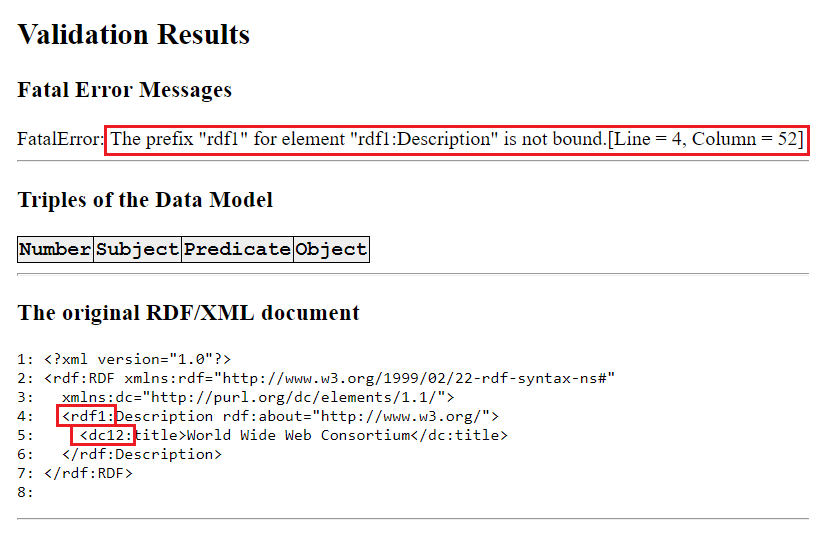
\includegraphics[scale=0.7,angle=0]{images/errorW3RDFValidator.png}
			\caption{\textbf{Validation results of the W3C RDF validation tool \cite{W3C:Validation:Online} after parsing an RDF/XML text, included two syntax errors.} The original RDF/XML document has two syntax errors since ``rdf1" and ``dc12" have no prefix declarations, but the results under ``Fatal Error Messages" show only the first found error and neglects the other.}
			\label{Fig:errorW3RDFValidator}
		\end{center}
	\end{figure}
\subsection{Several Serialization Formats Parsing Tools}

\par Next, the existing tools that validate more than one RDF serializations are checked. 
We have started with Jena RDF toolkit \cite{McBride:2002:JSW:613357.613755} which offers a validation service based on the ARP parser. 
It can be also used as a standalone program using a command-line or as an API integrated within another application.
Considering its powerful capability of validating numerous RDF serializations including RDF/XML, similarly, only the first encountered error is reported.

 \begin{figure}[ht]
		\begin{center}
			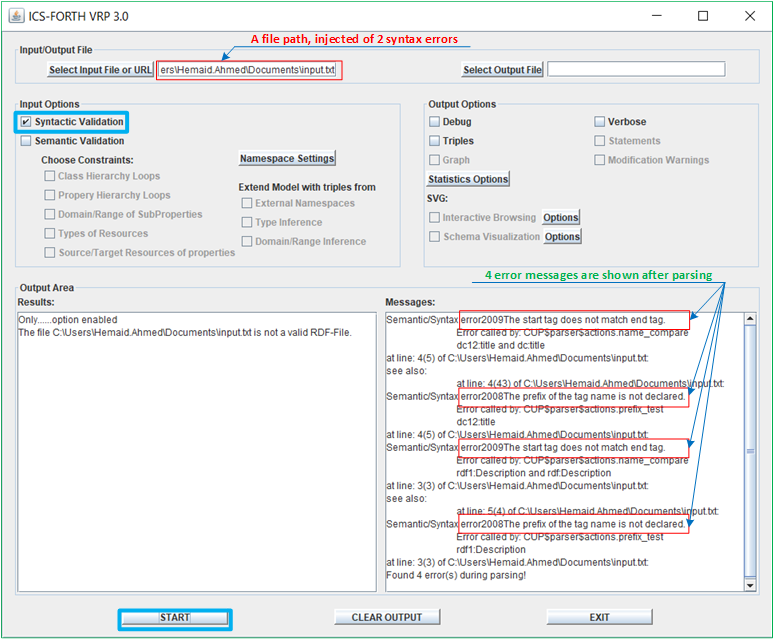
\includegraphics[scale=0.7,angle=0]{images/VRPErrorResult.png}
			\caption{\textbf{Results of Validating RDF Parser (VRP) \cite{karsten:Thesis:2000} after parsing an RDF/XML file.} Two errors are injected into the original RDF data. After the validation process, four error messages are shown, two of them are meaningful, whereas the other two messages have no meaning.}
			\label{Fig:VRPErrorResult}
		\end{center}
	\end{figure}
	
\vspace*{-\baselineskip}

\subsection{Classification of Parsing Approaches}

Approaches for validating various RDF serializations use the following core algorithms or methods as a significant part of their implementations. 
In the following, these core methods and their relations with concrete tools are discussed: 

\begin{itemize}[noitemsep] 

\item \textbf{ARP-parser-dependable approaches:} Both W3C RDF validation tool~\cite{W3C:Validation:Online} and RDF Validator and Converter~\cite{Mybluemix:Validation:Online} use the ARP parser of Jena framework \cite{McBride:2002:JSW:613357.613755}. 
The former validates only RDF/XML format whereas the later focuses more on triple-based serialization formats validating them and converting from one format to another. 

\item \textbf{N3-parser-dependable approaches:} This is mainly used by N3 parser~\cite{N3Parser:Online}, a JavaScript-based syntax validator, developed for checking the syntax of Turtle and N-Triple formats. 
The online version of IDLab Turtle Validator \cite{IDLab:Validation:Online} uses N3 parser and it is integrated as a NodeJS plug-in. 
The same approach was used to build a Turtle Editor with syntax validation in~\cite{petersenturtleeditor}. 
However, this approach is slow when parsing, and its behaviour is unpredictable when dealing with large files. 

\item \textbf{Shape expressions approaches:} In ~\cite{prud2014shape}, a Turtle parser was developed based on shape expressions \footnote{\url{https://www.w3.org/2001/sw/wiki/ShEx}}. 
Shape expressions describe the RDF graph based on regular expressions and validates RDF through declaring of constraints on the RDF data, if the declared constraints are violated, then RDF data is invalid, otherwise, it is valid. Furthermore, multiple tools we developed using the same approach in different programming languages, such as ShEx.js~\footnote{\url{https://github.com/shexSpec/shex.js}}, ShExJava~\footnote{\url{http://shexjava.lille.inria.fr/}}, Shaclex \footnote{\url{http://labra.weso.es/shaclex/}}, ShEx Ruby~\footnote{\url{https://ruby-rdf.github.io/shex/}}, PyShEx~\footnote {\url{https://github.com/hsolbrig/PyShEx}} built in JavaScript, Java, Scala, Ruby, Python, sequentially.

\item \textbf{Other parsing approaches:} Tools with another parsing method than the 3 listed above or unknown to us fall under this category. Raptor \footnote{\url{http://librdf.org/raptor/}} is a C-based open source library which includes parsers and serializers for a wide range of RDF serializations. 
It can be used as a standalone RDF parser. 
Also, Protege \footnote{\url{https://protege.stanford.edu/}}, is a free open source RDF editor, can work either as a desktop-based or a web-based application. 
It also supports several RDF serializations. Moreover, another variety of RDF parsers or tools: \cite{humfrey2010easyrdf},~\cite{RDF4J:Online},~\cite{krech2002rdflib} come
under  this category and the 2 last-mentioned parsers also failed to show more than the first syntax error.            
\end{itemize} 
\vspace*{-5mm}

The previous three approaches failed to list more than the first error at the same time. 
Moreover, an essential while processing a large number of RDF data is the performance, which is a weak point in the browser based tools such those implemented in JavaScript.

\section{Types of Error Messages}

Releasing user-friendly and meaningful error messages is of a great benefit to help the user to easily identify and correct the errors. 
\begin{itemize}
    \item \textbf{Non-expressive and meaningless error messages:} The parsing tools under the shape expressions approach like~\cite{prud2014shape} show less expressive and unfriendly error messages.
    \item \textbf{Expressive error and meaningful messages:} The parsing tools which utilize a ARP-parser-dependable approach like~\cite{N3Parser:Online},~\cite{Mybluemix:Validation:Online},~\cite{McBride:2002:JSW:613357.613755} or a N3-parser-dependable approach like~\cite{N3Parser:Online},~\cite{IDLab:Validation:Online},~\cite{petersenturtleeditor} are presenting more expressive and user-friendly error messages including its location in a proper way. 
    
\end{itemize}

\section{Error Recovery Approaches}
The existence of the automatic error recovery or correction feature is valuable to resolve from common syntax errors in RDF data.  Our survey of research papers and tools in relation to an auto-correction of RDF syntax errors shows that such a feature is not exit either theoretically or practically. %For example, a number of programming languages need a semicolon at the end of the line. 
%There are also few tools which can correct, such errors without the involvement of the programmer. 
%In the same way it will be useful to have this option of automatic correction after parsing of various serialization formats of RDF. 
However, Halilaj et al in \cite{Git4Voc:article} pointed out the need for this feature and explored its benefits.
Further, while searching other tools and approaches which have the same feature in other fields, \cite{AutoCorrection:Fix-it} was found.  \cite{AutoCorrection:Fix-it} reports about a Review Bot tool that can automatically review a source code using static analysis output and correct encountered syntax errors using the parser tree. Their approach is applicable in our case, but since a subset of common syntax errors are statically corrected in the current version of RDF-Doctor based on the collected error messages.    

\section{Summary}

Although there exist a number of tools developed over the years to deal with validation of RDF data from syntactic perspective, the majority of them fail in the first encountered error.
Moreover, several tools are limited only to the human users and do not provide any command-line or API interface.
Therefore, we foresee the need for a comprehensive approach able to identify all syntax errors at the same time and provide meaningful messages to help users to correct them.
In addition, a feature to automatically correct a number of common syntax errors is crucial to reduce time consumed for correction process.  

%after describing the actual issue, reviewing the state-of-art of research works, related to the same spot with pointing out the different approaches of RDF parsing and syntax checking, different types of error messages, and finally the approach of automatic error correction. 
%The outcome of this study is the RDF-Doctor. It is a parser that is generated with the help of the ANTLR parser generator. 
%Additionally, It is a Java\_based application to parse N-Triple and Turtle serialization formats; show a meaningful error messages; as well as, automatically recover from common syntax errors.    










